\DiaryEntry{Lattices, I}{2016-08-30}{Algebra}


\subsection{Background}\label{background}

A relation on a set \(X\) is a subset of \(X \times X\) (i.e the subset
for which the relation holds).

\subsubsection{Partial Orderings}\label{partial-orderings}

A relation \(P\) is a partial order of \(X\), if it fulfills the
following conditions:

\begin{itemize}
\item
  It is reflexive: \((a,a) \in P, \forall a \in X\).
\item
  It is antisymmetric: If \((a,b) \in P\) and \((b,a) \in P\), then
  \(a=b\)
\item
  It is transitive: If \((a,b) \in P\) and \((b,c) \in P\), then
  \((a,c) \in P\).
\end{itemize}

Note that this definition does \textbf{not} require that all elements of
X are lreated with each other; i.e.~some elements may not be related
with each other.

If a relation is \textbf{total}, then either \((a,b) \in P\) or
\((b,a) \in P\) for \textbf{all} \(a,b \in X\) - in other words, all
elements of the set can be compared with each other.

As an example of a partial ordering, consider the power set (the set of
all subsets) of the set \(X=\{a,b,c\}\). Then the power set are the
following sets: \[
\{\}, \{a\}, \{b\},\{c\}, \{a,b\}, \{a,c\}, \{b,c\}, \{a,b,c\}
\]

Set inclusion, denoted by \(\subseteq\) is a partial ordering: For
example, we have \(\{a\} \subseteq \{a,b\}\), but there is no relation
between \(\{a\}\) and \$\{b\} or between \(\{a\}\) and \(\{b,c\}\).

These relations (and their lack between certain elements) can be
visualised in a Hasse diagram as shown below.

\begin{figure}
\centering
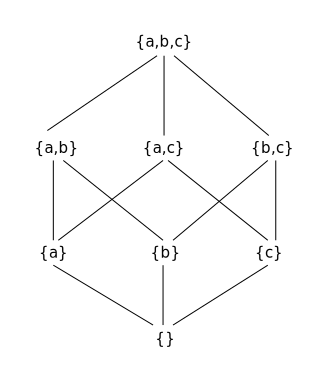
\includegraphics{images/lattices_01_1.png}
\caption{Page1}
\end{figure}

Another example is the partial order defined by \(a \leq b\) as
\(a | b\) with \(a,b \in \mathbb{N}\). This is reflexive, as \(a | a\)
holds fors all \(a,b\). If \(a|b\) and \(b|a\), then \(a=b\), so the
relation is antisymmetric, Finally, the relation is transitive, because
if \(m|n\) and \(n|p\), then \(m|p\).

If we consider the set \(X=\{1,2,3,4,6,8,12,24\}\) with this relation,
then we obtain the following Hasse diagram.

\begin{figure}
\centering
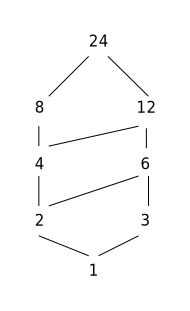
\includegraphics{images/lattices_01_2.png}
\caption{Page1}
\end{figure}
